\providecommand{\main}{..}
\documentclass[../cmpe-251-project-report.tex]{subfiles}
\externaldocument{1-introduction}
\externaldocument{2-dataset-properties}
\externaldocument{3-attribute-selection-ranking}
\externaldocument{4-clustering}
\externaldocument{6-actionable-conclusions}

\begin{document}
  \chapter{Predictors}
  With knowledge of the dataset's characteristics, different types of predictors were built to help determine whether a visitor will generate Revenue by making a purchase at Nozama's website. Three predictors, namely Random Forest (RF), Support Vector Machine (SVM), and \(k\)-nearest neighbours (\(k\)-NN).
  \section{Random Forests}
  A RF predictor was built first, as seen in \cref{fig:rf-workflow}, since its reliability gives a good baseline to evaluate other predictors on.
  \begin{figure}
    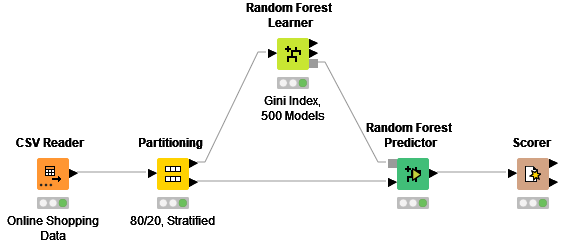
\includegraphics{img/rf-workflow.png}
    \caption{KNIME workflow used to build the RF predictor.}
    \label{fig:rf-workflow}
  \end{figure}
  \begin{figure}
    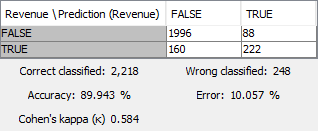
\includegraphics{img/rf-confusion-matrix.png}
    \caption{Confusion matrix of the RF predictor built.}
    \label{fig:rf-confusion-matrix}
  \end{figure}
  The prediction accuracy of \qty{89.9}{\percent} seen from the confusion matrix shown in \cref{fig:rf-confusion-matrix} is greater than the minimum prediction accuracy of \qty{84.5}{\percent} determined in \cref{ch:dataset-properties}. Then the RF predictor does provide value as an improvement over naively guessing that no visitor will generate Revenue.

  \section{Support Vector Machines}
  An SVM predictor was built next, as seen in \cref{fig:svm-workflow}, since the prediction attribute has two classes. But using any of the 3 kernel functions (polynomial, hypertangent, radial basis), results in a predictor that's less accurate than the RF predictor and sometimes doesn't meet the \qty{84.5}{\percent} threshold of naively guessing. This may be due to the lack of separation between the classes seen in \cref{subfig:svd-revenue-clustering}, resulting in the difficulty of a kernel function to map the data points into a space where there is sufficient separation between the classes.
  \begin{figure}
    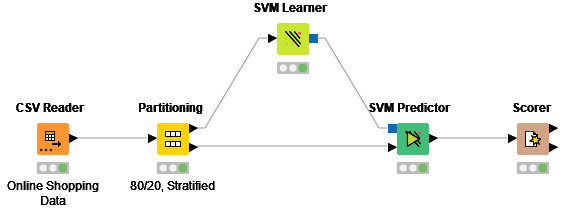
\includegraphics{img/svm-workflow.png}
    \caption{KNIME workflow used to build the SVM predictor.}
    \label{fig:svm-workflow}
  \end{figure}

  \section{\(k\)-nearest neighbours}
  \(k\)-NN was the last prediction method to consider, as built in \cref{fig:knn-workflow}, since cluster results from \cref{ch:clustering} indicated that it might be feasible to for a \(k\)-NN to have a higher prediction accuracy than the RF predictor.
  \begin{figure}
    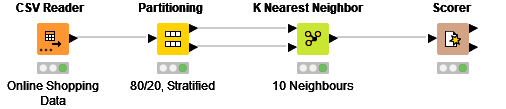
\includegraphics{img/knn-workflow.png}
    \caption{KNIME workflow used to build the \(k\)-NN predictor.}
    \label{fig:knn-workflow}
  \end{figure}
  \begin{figure}
    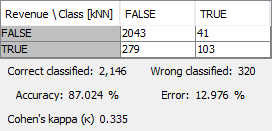
\includegraphics{img/knn-confusion-matrix.png}
    \caption{Confusion matrix of the \(k\)-NN predictor built.}
    \label{fig:knn-confusion-matrix}
  \end{figure}
  The prediction accuracy of \qty{87.0}{\percent} observed in the confusion matrix shown in \cref{fig:rf-confusion-matrix} is better than naively guessing all FALSE, but doesn't improve in the RF predictor. In retrospect, the non-existent separation between the blue and red data points in \cref{subfig:svd-revenue-clustering} imply that that the \(k\)-NN predictor would have a difficult time dealing with data points close tho the boundary between the two revenue classes.
\end{document}
